\documentclass[margin=5pt]{standalone}
\usepackage{pgfplots}
\usepgfplotslibrary{fillbetween,decorations.softclip}
\pgfplotsset{compat = newest}
\begin{document}
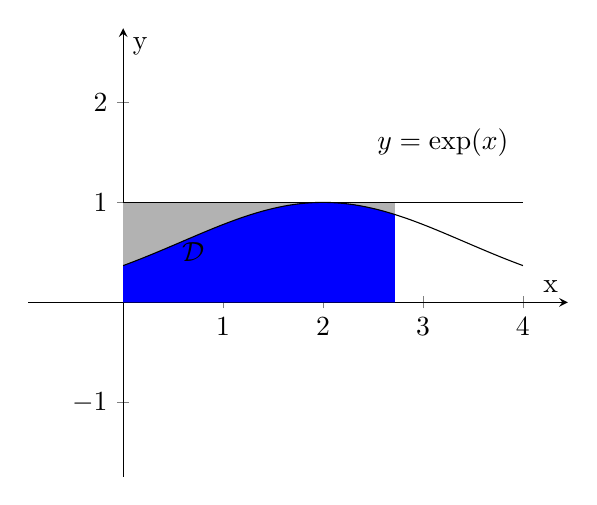
\begin{tikzpicture}
  \pgfdeclarelayer{pre main}
  \pgfsetlayers{pre main,main}
  \begin{axis}[
      axis lines = middle,
      axis equal,
      enlargelimits,
      domain  = 0:4,
      xlabel  = {x},
      ylabel  = {y},
      xmin    = -0.5,
      xmax    = 4,
      ymin    = -1,
      ymax    = 2,
      samples = 300,
      mark    = none,
    ]
    \pgfonlayer{pre main}
    \fill[black!30] (0,0) rectangle (e,1);
    \endpgfonlayer
    \addplot [name path=ln, thin]  {exp(-(x - 2)^2/4)};
    \addplot [thin]  {1};
    \addplot [name path=null, draw=none]  {0};
    \addplot[color=blue] fill between[of=null and ln,
      soft clip={domain=0:e}];
    \node at (0.7,0.5) {$\mathcal{D}$};
    \node at (3.2,1.6) {$y = \exp(x)$};
  \end{axis}
\end{tikzpicture}
\end{document}